\chapter{Sistemas}

Un sistema es una operación que transforma una señal de entrada $x$ en una señal de salida $y$.
Puede modificar la señal de diversas maneras, según la naturaleza de la transformación.

\begin{mdframed}[style=DefinitionFrame]
    \begin{defn}
    \end{defn}
    \cusTi{Transformación asociada a un sistema}
    \cusTe{}
    \[
        \fx[y]{t} = \fx[T]{\fx[x]{t}}
    \]
\end{mdframed}

\begin{itemize}
    \item
    \textbf{Modificación de amplitud:}
    Puede escalar los valores de la señal, amplificándolos o atenuándolos.
    \item
    \textbf{Modificación en tiempo:}
    Puede desplazar la señal, invertirla temporalmente o comprimirla.
    \item
    \textbf{Filtrado:}
    Puede atenuar o eliminar ciertas componentes de frecuencia de la señal.
    \item
    \textbf{Integración y derivación:}
    Puede aplicar acumuladores o destacar cambios de una señal continua.
    \item
    \textbf{No lineales:}
    La distorción introduce frecuencias que no existían.
    La modulación cambia la forma de la señal.
\end{itemize}

\section{Clasificación de sistemas}

\begin{mdframed}[style=DefinitionFrame]
    \begin{defn}
    \end{defn}
    \cusTi{Sistema lineal}
    \cusTe{Un sistema es lineal si se puede aplicar el principio de superposición:}
    \[
        \fx[T]{a \, \fx[x_1]{t} + b \, \fx[x_2]{t}} = a \, \fx[y_1]{t} + b \, \fx[y_2]{t}
    \]
\end{mdframed}

\begin{mdframed}[style=DefinitionFrame]
    \begin{defn}
    \end{defn}
    \cusTi{Sistema invariante en el tiempo}
    \cusTe{Un sistema es invariante en el tiempo si su comportamiento no cambia con el tiempo.}
    \[
        \fx[T]{\fx[x]{t-t_0}} =\fx[y]{t-t_0}
    \]
\end{mdframed}

\begin{mdframed}[style=DefinitionFrame]
    \begin{defn}
    \end{defn}
    \cusTi{Sistema estable}
    \cusTe{Un sistema es estable si para una entrada acotada en amplitud, la salida también es acotada.}
\end{mdframed}

\begin{mdframed}[style=DefinitionFrame]
    \begin{defn}
    \end{defn}
    \cusTi{Sistema causal}
    \cusTe{Un sistema es causal o no anticipativo si la salida no comienza antes de aplicar la entrada.}
\end{mdframed}

\section{Función de transferencia}

La función de transferencia es una herramienta fundamental para el análisis de sistemas lineales e invariantes en el tiempo (LTI).
Describe cómo el sistema modifica las diferentes componentes de frecuencia de una señal.
Permite estudiar el comportamiento del sistema sin necesidad de resolver la ecuación diferencial que lo define.
Representa la relación entre la entrada y la salida del sistema en términos de frecuencia compleja.

\begin{mdframed}[style=DefinitionFrame]
    \begin{defn}
    \end{defn}
    \cusTi{Función de transferencia}
    \cusTe{Dado un sistema lineal e invariante en el tiempo se define la función de transferencia}
    \[
        \fx[H]{s} = \frac{\fx[Y]{s}}{\fx[X]{s}}
    \]
    donde $\fx[X]{s}$ e $\fx[Y]{s}$ son los espectros de las señales de entrada y salida, y $s = \sigma + \iu \omega$ la variable de Laplace.
\end{mdframed}

La parte real, $\sigma$, determina el crecimiento o decrecimiento exponencial.
Mientras que la parte imaginaria, $\omega$, determina la frecuencia angular de la señal.
Evaluar $\sigma = 0$ resulta útil porque permite estudiar cómo responde el sistema a señales senoidales.

El análisis de sistemas se facilita enormemente al estudiar su comportamiento frente a una señal compleja exponencial.
La señal $\fx[x]{t} = e^{\iu \omega t}$ es una \emph{autofunción} de los sistemas LTI.
Esto significa que la salida del sistema será la misma señal multiplicada por una constante compleja que depende de la frecuencia, pero no del tiempo.
Esta constante es precisamente la función de transferencia, que describe cómo se modifican la amplitud y la fase de cada componente frecuencial.
Y la expresión encontrada a partir de esta situación particular, es válida para cualquier señal de entrada.

\begin{mdframed}[style=PropertyFrame]
    \begin{prop}
        \label{prop:funcionDeTransferencia}
    \end{prop}
    Si un sistema LTI es alimentado con una señal de entrada $\fx[x]{t} = e^{\iu \omega \, t}$ entonces
    \[
        \fx[H]{\iu \omega} = \frac{\fx[y]{t}}{\fx[x]{t}}
    \]
\end{mdframed}

\section{Espectro bilateral}

El espectro bilateral es una representación que muestra la distribución de las componentes de frecuencia de una señal.
Indica el aporte en amplitud y en fase de cada frecuencia para formar la totalidad de la señal.

En la realidad solo existen frecuencias mayores a cero.
Las señales reales pueden ser representadas por cosenos, que son funciones pares.
Por esto, el signo de su argumento (dado por el signo de la frecuencia) no afecta la representación.
\[
    \fx[\cos]{\omega \, t + \varphi} = \fx[\cos]{- \omega \, t - \varphi}
\]

Pero al usar modelos matemáticos que tienen un dominio complejo es necesario considerar las frecuencias negativas, pues
\[
    e^{\iu (\omega \, t + \varphi)} \neq e^{- \iu (\omega \, t + \varphi)}
\]

Esto se evidencia con la siguiente propiedad de los números complejos.
Podemos representar una señal senoidal simple de argumento real como una suma de exponenciales de argumento complejo según:
\[
    \fx[\cos]{\omega \, t + \varphi} = \frac{e^{\iu (\omega \, t + \varphi)} + e^{- \iu (\omega \, t + \varphi)}}{2}
\]

A su vez, las señales reales pueden ser representadas por una suma de senoidales simples.
En ese desarrollo, eventualmente podría haber sumandos que sean senos o cosenos de amplitud negativa.
Pero por convención, es necesario reemplaar estos sumandos por el \textbf{coseno positivo} equivalente mediante un defasaje arbitrario.

El espectro bilateral consiste en dos gráficos que representan la \textbf{magnitud} y la \textbf{fase} que tiene cada una de las exponenciales simples de diferente \textbf{frecuencia} que forman la señal.

Si la señal tiene algún sumando constante, se puede representar como un coseno de frecuencia nula:
\[
    c = c \, \fx[\cos]{\omega \, t + \varphi} \text{ con } \omega = 0 \land \varphi = 0
\]

Por lo tanto, el gráfico de magnitud va a tener la totalidad de la componente constante en $\omega = 0$.
Pero para las demás componentes $\omega \neq 0$, se va a tener la mitad de la amplitud ya que se grafica el espectro dado por las exponenciales.

\subsection{Simetría hermitiana}

Se tiene un sistema LIT que se exita con la señal
\[
    \fx[x]{t} = A_x \, \fx[\cos]{\omega_x \, t + \varphi_x}
\]

Podemos asumir entonces, que la salida va a ser una señal senoidal de igual frecuencia.
Pero la amplitud y fase eventualmente se verán modificadas.
\[
    \fx[y]{t} = A_y \, \fx[\cos]{\omega_x \, t + \varphi_y}
\]

La función de transferencia estará dada por
\[
    \fx[H]{\iu \omega} = \norm{\fx[H]{\iu \omega}} \, e^{\iu \, \fx[\arg]{\fx[H]{\iu \omega}}}
\]
tal que
\[
    \fx[y]{t} = \fx[H]{\iu \omega} \, \fx[x]{t}
\]

Sabiendo que
\[
    z + \conj{z} = 2 \, \norm{z} \fx[\cos]{\fx[\arg]{z}}
    = \norm{z} e^{\iu \fx[\arg]{z}} + \norm{z} e^{- \iu \fx[\arg]{z}}
\]
podemos escribir la señal de entrada como
\[
    \fx[x]{t} = \frac{A_x}{2} e^{\iu \inParentheses{\omega_x \, t + \varphi_x}}
    + \frac{A_x}{2} e^{- \iu \inParentheses{\omega_x \, t + \varphi_x}}
\]

Dado que el sistema es lineal, pordemos aplicar superposición.
Osea que la transformación a todo el espectro es equivalente a la transformación de cada frecuencia:
\begin{align*}
    \fx[y]{t} & = \sum_{\nth=1}^{2} \fx[H]{\iu \omega_\nth}
    \, \alpha_\nth
    \, e^{\iu \inParentheses{\omega_\nth t + \varphi_\nth}}
    \\
    & = \sum_{\nth=1}^{2} \norm{\fx[H]{\iu \omega_\nth}}
    \, \alpha_\nth
    \, e^{\iu \inParentheses{\omega_\nth t + \varphi_\nth + \fx[\arg]{\fx[H]{\iu \omega_\nth}}}}
\end{align*}

La señal de salida queda luego dada por
\begin{multline*}
    \fx[y]{t} = \norm{\fx[H]{\iu \omega_x}}
    \, \frac{A_x}{2}
    \, e^{\iu \inParentheses{\omega_x t + \varphi_x + \fx[\arg]{\fx[H]{\iu \omega_x}}}}
    \\
    + \norm{\fx[H]{- \iu \omega_x}}
    \, \frac{A_x}{2}
    \, e^{\iu \inParentheses{- \omega_x t - \varphi_x + \fx[\arg]{\fx[H]{- \iu \omega_x}}}}
\end{multline*}

Dado que la señal de entrada es real, la señal de salida debe tener parte imaginaria nula:
\begin{equation*}
    \fx[x]{t} \in \setR \implies \fx[\Im]{\fx[y]{t}} = 0
\end{equation*}

A saber, la parte imaginaria de un complejo es:
\begin{equation*}
    \fx[\Im]{z} = \fx[\Im]{\norm{z} \, e^{\iu \, \fx[\arg]{z}}}
    = \norm{z} \, \fx[\sin]{\fx[\arg]{z}}
\end{equation*}

Igualando la parte imaginaria de $\fx[y]{t}$ a cero, se obtiene la siguiente ecuación:
\begin{multline*}
    \norm{\fx[H]{\iu \omega_x}}
    \, \frac{A_x}{2}
    \, \fx[\sin]{\omega_x t + \varphi_x + \fx[\arg]{\fx[H]{\iu \omega_x}}}
    =
    \\
    =
    - \norm{\fx[H]{- \iu \omega_x}}
    \, \frac{A_x}{2}
    \, \fx[\sin]{- \omega_x t - \varphi_x + \fx[\arg]{\fx[H]{- \iu \omega_x}}}
\end{multline*}

Dado que $\fx[\sin]{-\varphi} = - \fx[\sin]{\varphi}$ se tiene:
\begin{multline*}
    \norm{\fx[H]{\iu \omega_x}}
    \, \fx[\sin]{\omega_x t + \varphi_x + \fx[\arg]{\fx[H]{\iu \omega_x}}}
    =
    \\
    =
    \norm{\fx[H]{- \iu \omega_x}}
    \, \fx[\sin]{\omega_x t + \varphi_x - \fx[\arg]{\fx[H]{- \iu \omega_x}}}
\end{multline*}

De manera que para que se cumpla la igualdad, el espectro de frecuencias tiene que tener amplitud par y fase impar.

\begin{mdframed}[style=PropertyFrame]
    \begin{prop}
    \end{prop}
    \cusTi{Simetría hermitiana}
    \cusTe{Un sistema lineal e invariante en el tiempo exitado por una señal senoidal simple de frecuencia $\omega_x$ verifica:}
    \begin{align*}
        \norm{\fx[H]{\iu \omega_x}} & = \norm{\fx[H]{- \iu \omega_x}}
        \\
        \fx[\arg]{\fx[H]{\iu \omega_x}} & = - \fx[\arg]{\fx[H]{- \iu \omega_x}}
    \end{align*}
\end{mdframed}

\begin{mdframed}[style=ExampleFrame]
    \begin{example}
        \label{ej:hermitiana}
    \end{example}
    Una señal periódica $\fx[x]{t}$ con nivel DC nulo y período $T_0$ se puede representar con una suma infinita de exponenciales complejas.
    Sus coeficientes $c_k$ están dados para $k>0$ por:
    \[
        c_k = \frac{4 \iu^k}{k}
    \]

    Obtener el espectro de salida para un sistema con la siguiente función de transferencia:
    \[
        \fx[H]{\iu \omega} =
        \pulse{f \, T_0}{5}
        \, e^\frac{\iu \pi \, f \, T_0}{4}
    \]
    
    \concept{Resolución:}
    
    La sucesión dada es la siguiente:
    \begin{align*}
        \inBraces{c_k}
        & = \inBraces{\cdots \frac{-4}{5 \iu} ; -1 ; \frac{4}{3 \iu} ; 2 ; \frac{-4}{\iu} ; 4 \iu ; -2 ; \frac{-4}{3 \iu} ; 1 ; \frac{4}{5 \iu} \cdots}
        \\
        & = \inBraces{\cdots \frac{4 \iu}{5} ; -1 ; \frac{-4 \iu}{3} ; 2 ; 4 \iu ; 4 \iu ; -2 ; \frac{4 \iu}{3} ; 1 ; \frac{-4 \iu}{5} \cdots}
    \end{align*}

    Pero según el enunciado, la señal $\fx[x]{t}$ está dada por aquellos coeficientes donde $k>0$:
    \[
        \inBraces{c_k} = \inBraces{4 \iu ; -2 ; \frac{4 \iu}{3} ; 1 ; \frac{-4 \iu}{5} \cdots}
    \]

    Notar que el espectro bilateral de $\fx[x]{t}$ está dado por el módulo y el argumento de los coeficientes.
    En el desarrollo en series de $\fx[x]{t}$, la exponencial que tiene la variable temporal es una oscilación simple.
    Son los coeficientes $c_k$ los que determinan el aporte de la magnitud y la fase de cada frecuencia.
    Por ejemplo, para $k=5$ se tiene que el sumando es
    \[
        c_5 \, e^{\iu \omega_0 \, t}
        = \frac{4 \iu}{5} \, e^{\iu \omega_0 \, t}
        = \frac{4}{5} \, e^{\iu \frac{\pi}{2}} \, e^{\iu \omega_0 \, t}
        = \frac{4}{5} \, e^{\iu \inParentheses{\omega_0 \, t + \frac{\pi}{2}}}
    \]
    haciéndose evidente que el módulo y el argumento de $c_5$ son iguales al módulo y la fase de todo el sumando.

    Por lo tanto, el espectro de la señal $\fx[x]{t}$ es
    \begin{center}
        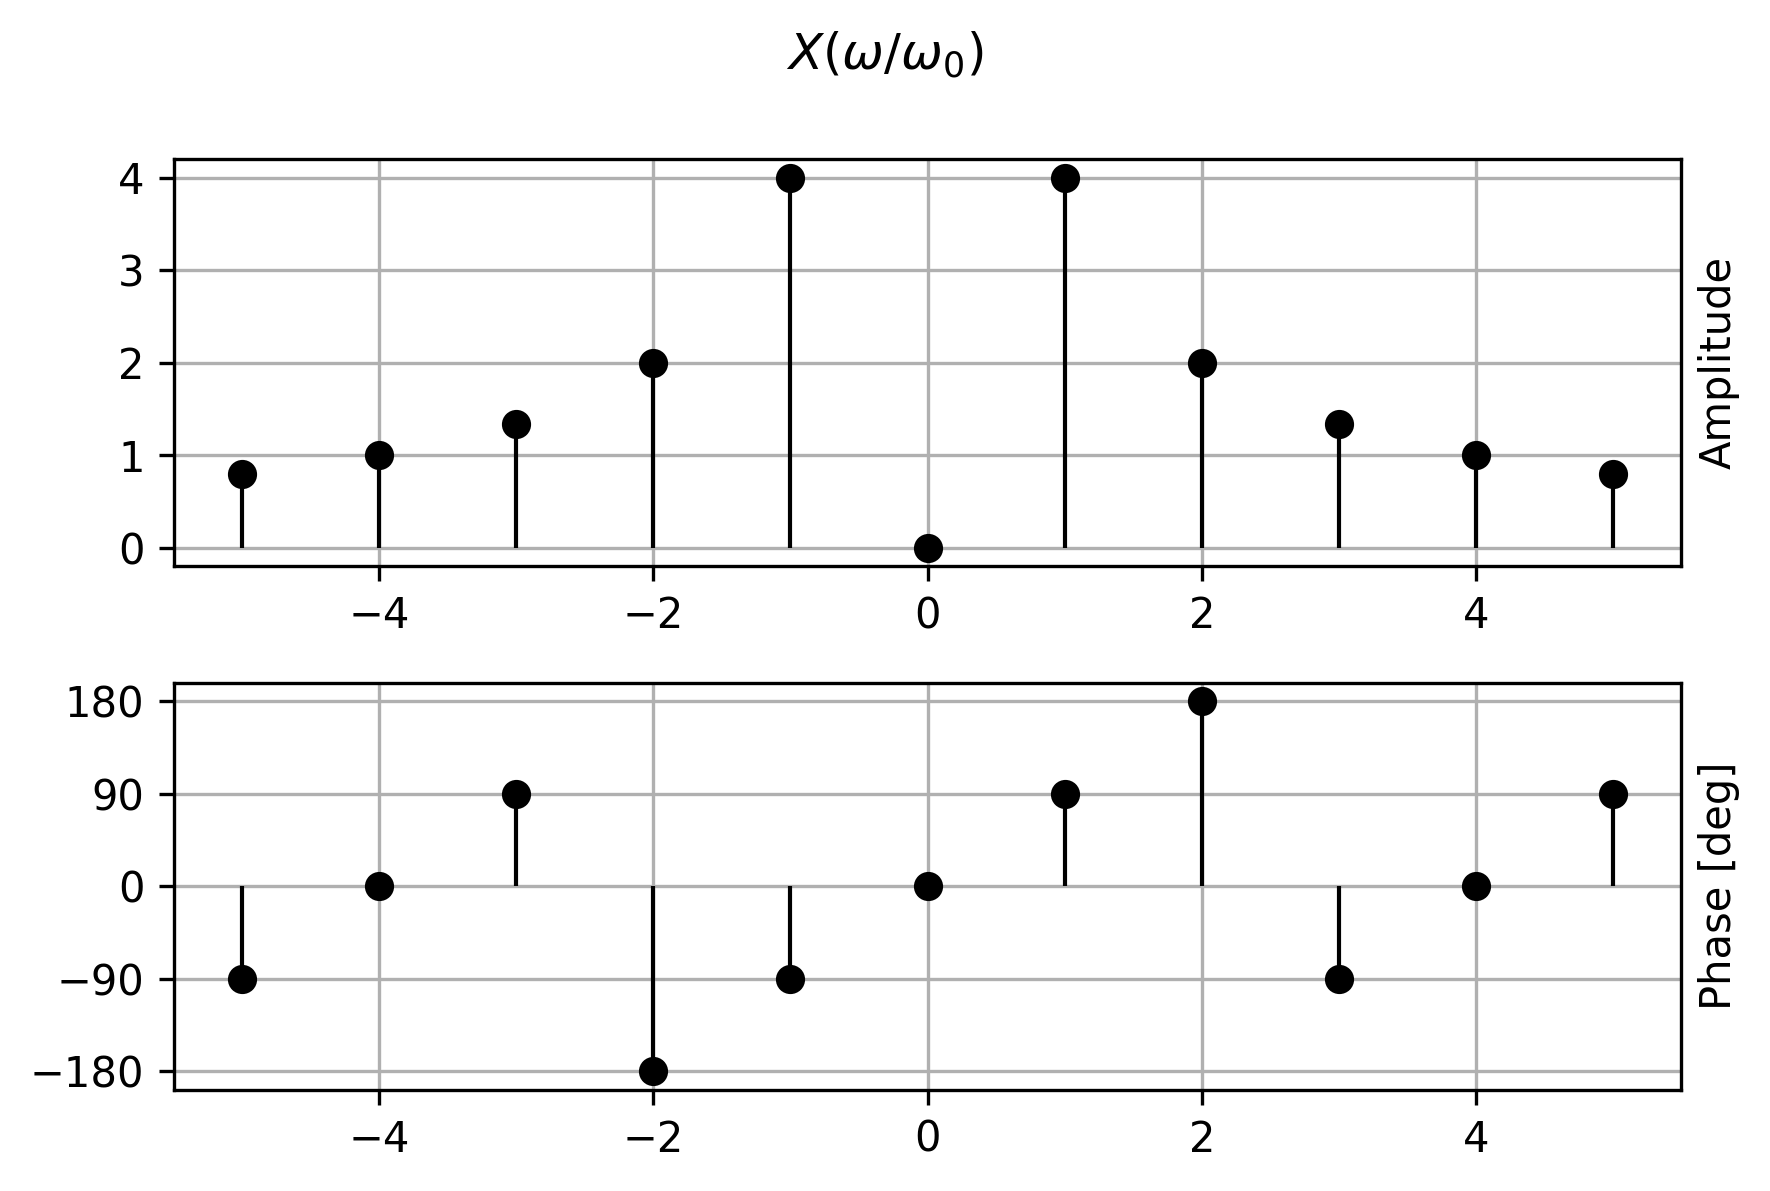
\includegraphics[width=\linewidth]{./images/ej_siemtria_hermitiana_x.png}
    \end{center}

    La función de transferencia es:
    \[
        \fx[H]{\iu \omega} = \pulse{\omega}{5 \, \omega_0} \, e^{-\frac{\iu \, \pi \, \omega}{4 \, \omega_0}}
    \]
    pues
    \[
        \left\{
        \begin{aligned}
            & \frac{f \, T_0}{5}
            = \frac{1}{5} \, f \, T_0
            = \frac{1}{5} \, \frac{\omega}{2 \pi} \, \frac{2 \pi}{\omega_0}
            = \frac{\omega}{5 \, \omega_0}
            \\[1em]
            & \frac{\iu \pi \, f \, T_0}{4}
            = \frac{\iu \pi}{4} \, f \, T_0
            = \frac{\iu \pi}{4} \, \frac{\omega}{2 \pi} \, \frac{2 \pi}{\omega_0}
            = \frac{\iu \, \pi \, \omega}{4 \, \omega_0}
        \end{aligned}
        \right.
    \]

    Luego:
    \begin{gather*}
        \norm{\fx[H]{\omega}} =
        \left\{
        \begin{aligned}
            & 1 \text{ si } \omega \in [-2 \, \omega_0 ; 2 \, \omega_0]
            \\
            & 0 \text{ si } \omega \notin [-2 \, \omega_0 ; 2 \, \omega_0]
        \end{aligned}
        \right.
        \\[1em]
        \fx[\arg]{\fx[H]{\omega}} =
        - \frac{\pi \, \omega}{4 \, \omega_0}
    \end{gather*}

    Y el espectro de la función de transferencia es:
    \begin{center}
        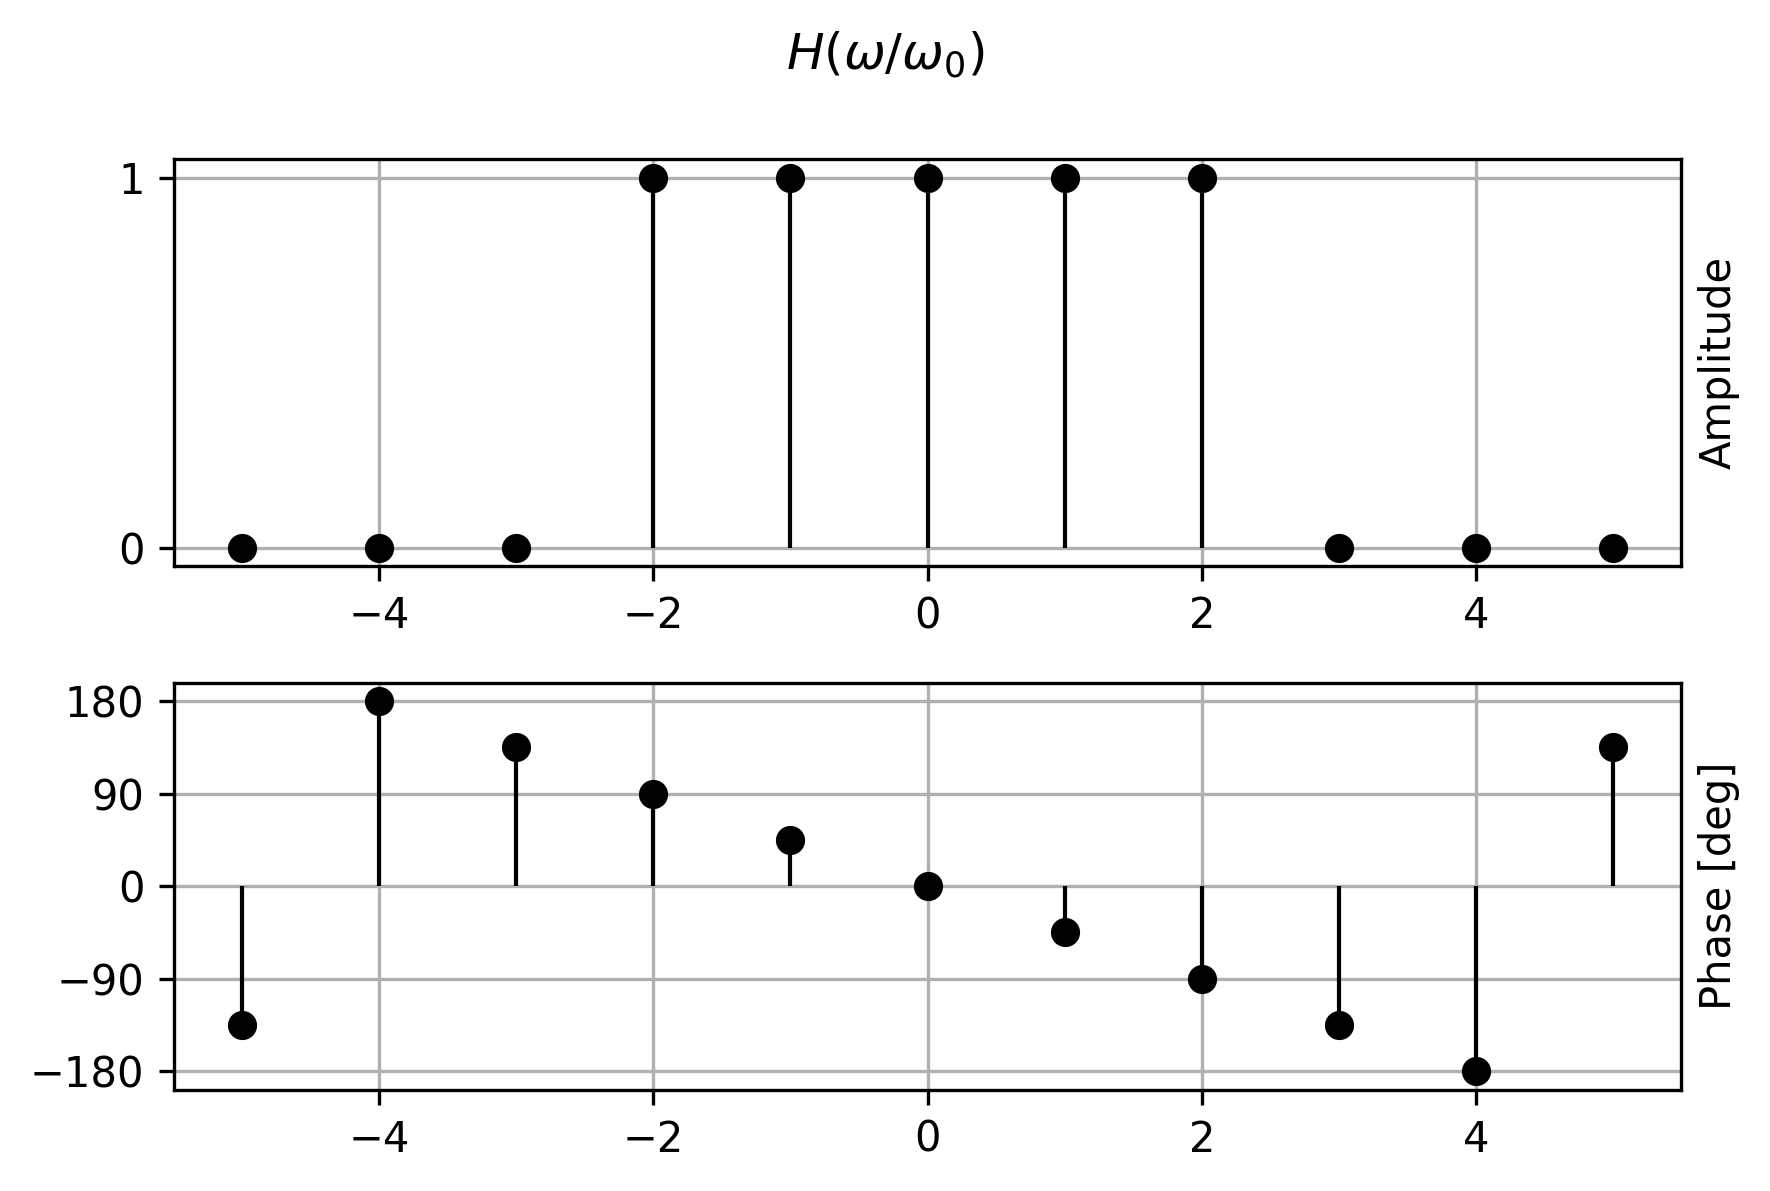
\includegraphics[width=\linewidth]{./images/ej_siemtria_hermitiana_h.png}
    \end{center}

    Multiplicando las magnitudes y sumando las fases de $\fx[x]{t}$ con las de $\fx[H]{\omega}$, se obtiene:
    \begin{center}
        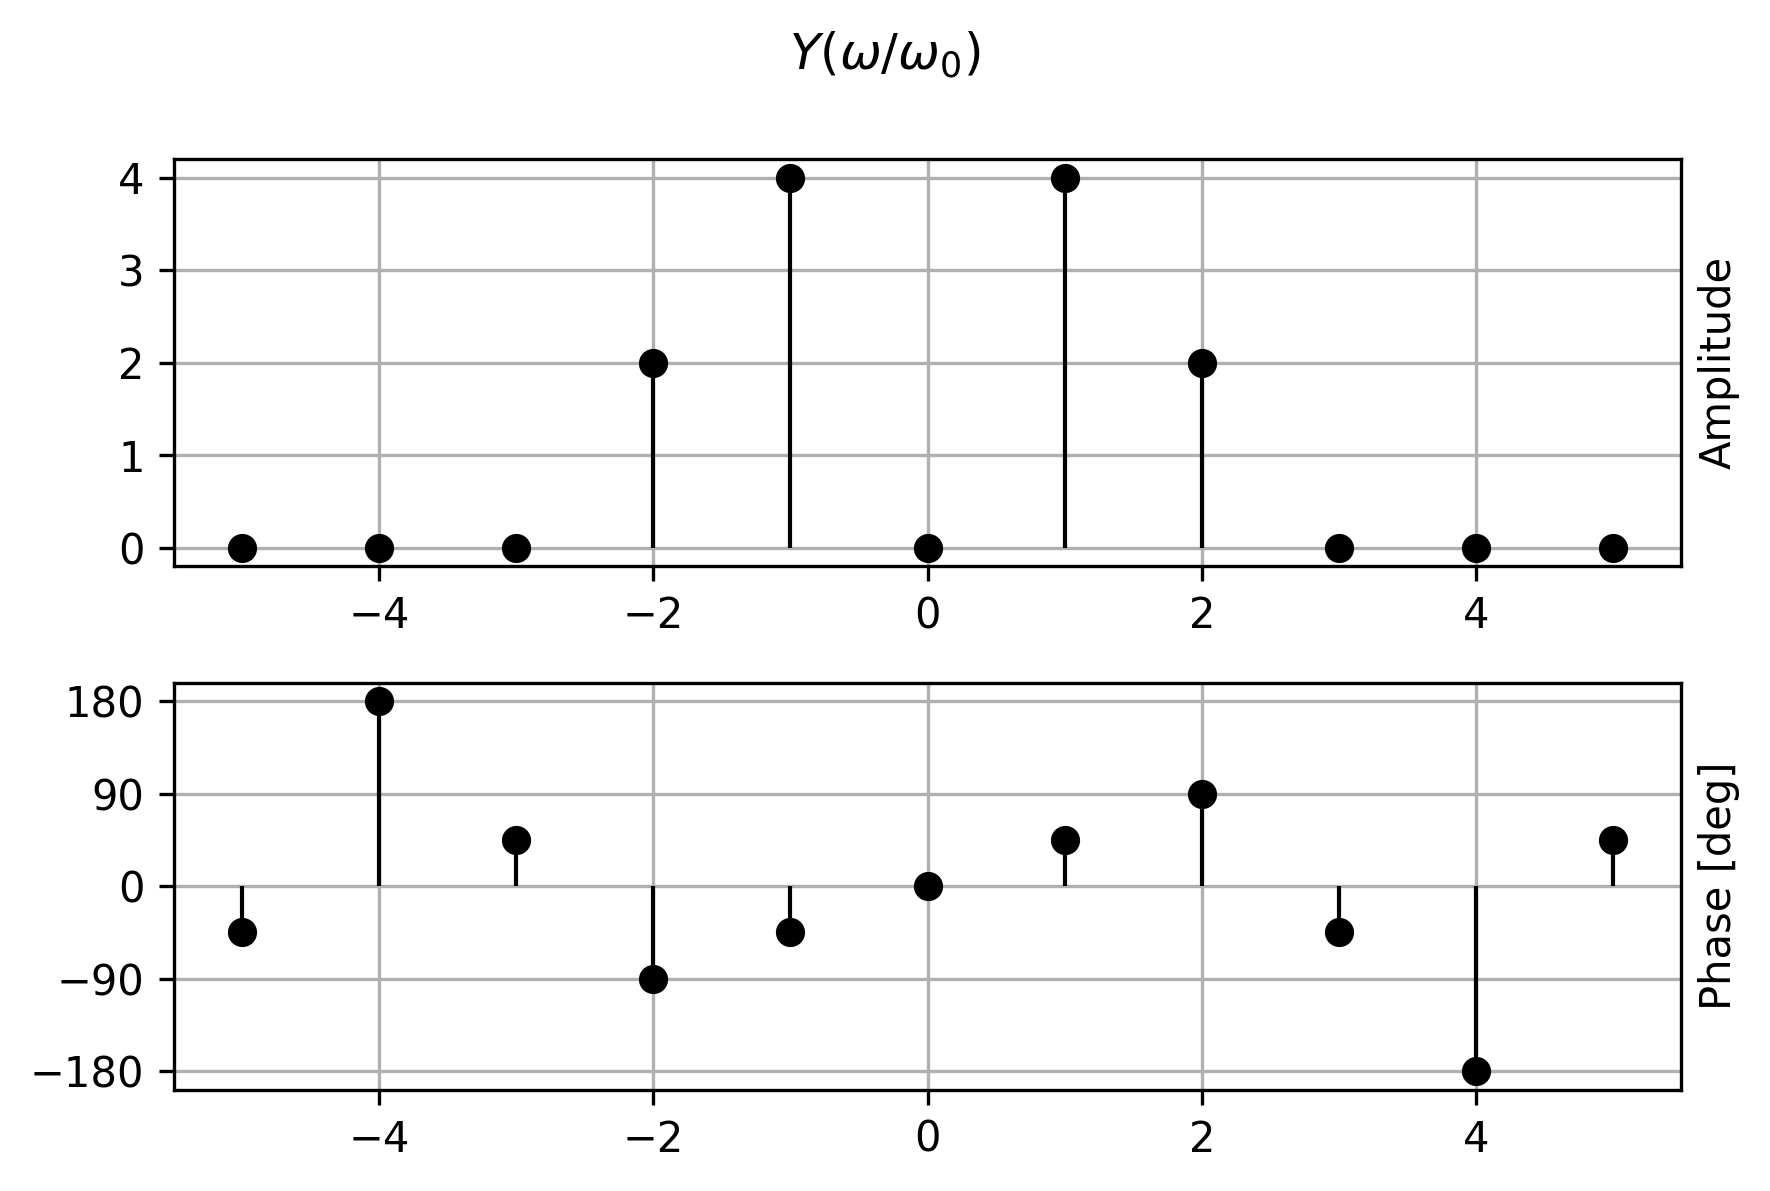
\includegraphics[width=\linewidth]{./images/ej_siemtria_hermitiana_y.png}
    \end{center}
\end{mdframed}

\section{Fase lineal}

Al pasar una señal por cualquier sistema LTI, cada componente frecuencial sufre un defasaje.
Este cambio en la fase genera un retraso temporal en el espectro de la señal, conocido como retardo de grupo.

\begin{mdframed}[style=DefinitionFrame]
    \begin{defn}
        \label{defn:groupDelay}
    \end{defn}
    \cusTi{Retardo de grupo}
    \[
        \fx[\tau_g]{\omega} = - \frac{\dif}{\dif \omega} \fx[\varphi]{\omega}
    \]
    donde
    \[
        \fx[\varphi]{\omega} = \fx[\arg]{\fx[H]{\omega}}
    \]
\end{mdframed}

Si el sistema es de \emph{fase lineal}, el tiempo de retraso por defasaje es el mismo para todas las frecuencias.
El gráfico de $\fx[\varphi]{\omega}$ resulta ser una recta y su pendiente es el retardo de grupo.

A partir de la ecuación de la recta
\[
    \fx[\varphi]{\omega} = - \tau_g \inParentheses{\omega - \omega_0} + \varphi_0
\]
vemos que el defasaje es proporcional a la frecuencia, y $\tau_g$ es el factor de proporción.
Reacomodando esta expresión, se obtiene la siguiente relación.

\begin{mdframed}[style=PropertyFrame]
    \begin{prop}
        \label{prop:groupDelay}
    \end{prop}
    Para un sistema LTI con fase lineal se cumple que
    \[
        \tau_g = - \frac{\Delta \varphi}{\Delta \omega}
    \]
\end{mdframed}

\begin{mdframed}[style=ExampleFrame]
    \begin{example}
    \end{example}
    Analicemos, del ejemplo \ref{ej:hermitiana}, el defasaje producido por un filtro de fase lineal:
    \[
        \fx[\varphi]{\omega} = - \frac{\pi \, \omega}{4 \, \omega_0}
    \]

    El retardo de grupo está dado, según la definición \ref{defn:groupDelay}, por:
    \[
        \tau_g = \frac{\pi}{4 \, \omega_0}
    \]

    Recordemos que $\omega_0$ era una constante definida en el enunciado como un parámetro del filtro.
    Para efectos prácticos podemos suponer que $f_0 = \kHz$, luego
    \[
        \omega_0 = 2 \, \pi \, \SI{1000}{\radian\per\second}
    \]
    y el retardo de grupo es
    \[
        \tau_g = \SI{0.125}{\milli\second}
    \]

    A continuación se tiene un gráfico de las componentes senoidales de $\fx[H]{\iu \omega}$ con y sin retraso.
    Vemos que ambas frecuencias retrasan $\SI{0.125}{\milli\second}$.
    Pero este corrimiento temporal implica un defasaje distinto para cada frecuencia.

    \begin{center}
        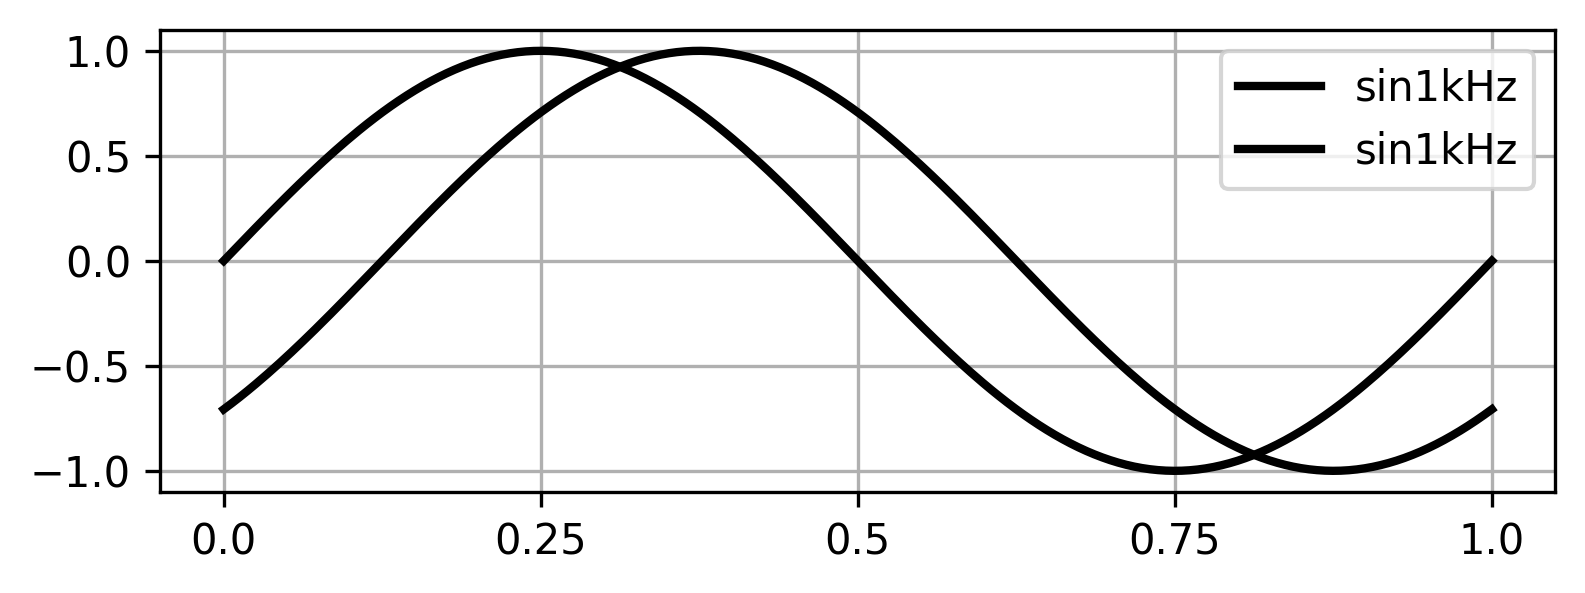
\includegraphics[width=\linewidth]{./images/ej_fase_lineal_1.png}
        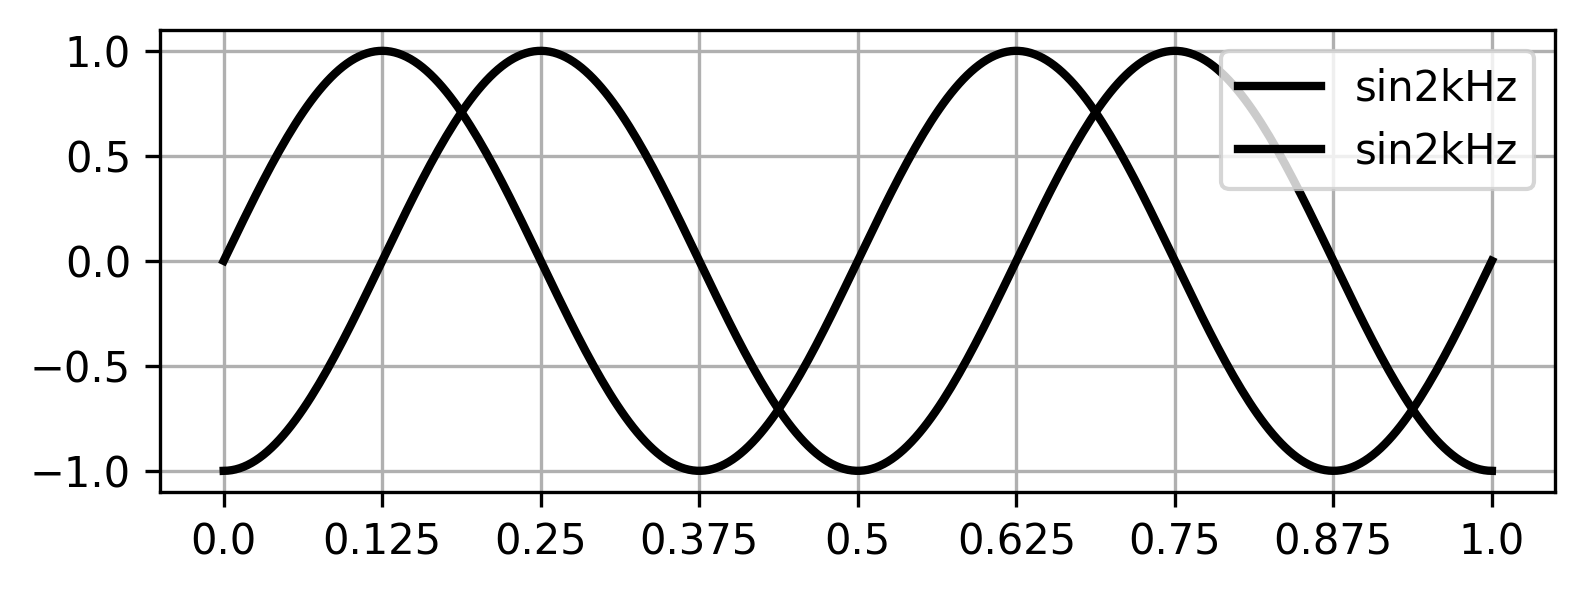
\includegraphics[width=\linewidth]{./images/ej_fase_lineal_2.png}
    \end{center}

    Verifiquemos que el retardo de fase es igual para todas las frecuencias, además de las 2 graficadas.
    Según la propiedad \ref{prop:groupDelay}, para 2 frecuencias cualquiera y sus respectivos retardos, la proporción es constante:
    \begin{align*}
        \tau_g
        & = \frac{\frac{\pi}{2} - \frac{\pi}{4}}{2 \pi \inParentheses{\kHz[2] - \kHz[1]}}
        \\[1em]
        & = \frac{\frac{3}{4} \pi - \frac{\pi}{4}}{2 \pi \inParentheses{\kHz[3] - \kHz[1]}}
        \\[1em]
        & = \frac{\frac{3}{4} \pi - \frac{\pi}{2}}{2 \pi \inParentheses{\kHz[3] - \kHz[2]}}
        \\[1em]
        & = \SI{0.125}{\milli\second}
    \end{align*}
\end{mdframed}

\section{Respuesta al impulso}

Otra forma de caracterizar un sistema lineal e invariante en el tiempo (LTI) es a través de su respuesta al impulso.
Esta se define como la salida del sistema cuando la entrada es el impulso de Dirac, denotado por $\fx[\delta]{t}$.

Si un sistema LTI recibe como entrada la función $\fx[\delta]{t}$ y genera una salida $\fx[h]{t}$, se dice que $\fx[h]{t}$ es la respuesta al impulso del sistema.

\begin{mdframed}[style=DefinitionFrame]
    \begin{defn}
    \end{defn}
    \cusTi{Respuesta al impulso}
    \cusTe{Dado un sistema LTI representado por una transformación $T$, su respuesta al impulso es}
    \begin{equation*}
        \fx[h]{t} = \fx[T]{\fx[\delta]{t}}
    \end{equation*}
\end{mdframed}

En el capítulo \ref{chapter:convolucion} se muestra que esta función contiene la información necesaria para describir el comportamiento del sistema ante cualquier entrada.

\section{Sistemas típicos}

El procedimiento para determinar la función de transferencia consiste en aplicar al sistema una entrada de la forma \( \fx[x]{t} = e^{\iu \omega t} \).
De esta forma, es posible obtener la salida correspondiente \( \fx[y]{t} \) para luego calcular el cociente
\[
    \fx[H]{\iu \omega} = \frac{\fx[y]{t}}{\fx[x]{t}}
\]

Para calcular la respuesta al impulso por definición, hay que evaluar $\fx[x]{t} = \fx[\delta]{t}$.
Así, la salida obtenida será
\[
    \fx[y]{t} = \fx[h]{t}
\]

\subsection{Multiplicador por constante}

Este sistema \textbf{multiplica} la señal por una constante:
\[
    \fx[y]{t} = C \, \fx[x]{t}
\]

Si $\fx[x]{t} = e^{\iu \omega t}$, la salida será
\[
    \fx[y]{t} = C \, e^{\iu \omega t}
\]
luego, la \textbf{respuesta en frecuencia} es
\[
    \fx[H]{\iu \omega} = C
\]

La \textbf{respuesta al impulso} está dada por
\[
    \fx[h]{t} = C \, \fx[\delta]{t}
\]

\subsection{Retardador}

Este sistema \textbf{desplaza en el tiempo} la señal una cantidad $t_0$ hacia el futuro:
\[
    \fx[y]{t} = \fx[x]{t - t_0}
\]

Si $\fx[x]{t} = e^{\iu \omega t}$, la salida será
\begin{align*}
    \fx[y]{t}
    & = e^{\iu \, \omega \, (t - t_0)}
    \\
    & = e^{-\iu \, \omega \, t_0} \, e^{\iu \omega t}
\end{align*}
luego, la \textbf{respuesta en frecuencia} es
\[
    \fx[H]{\iu \omega} = e^{- \iu \, \omega \, t_0}
\]

La \textbf{respuesta al impulso} está dada por
\[
    \fx[h]{t} = \fx[\delta]{t - t_0}
\]

\subsection{Derivador}

Este sistema \textbf{devuelve la derivada} de la señal:
\[
    \fx[y]{t} = \frac{\dif}{\dif t} \fx[x]{t}
\]

Si $\fx[x]{t} = e^{\iu \omega t}$, la salida será
\[
    \fx[y]{t} = \iu \omega \, e^{\iu \omega t}
\]
luego, la \textbf{respuesta en frecuencia} es
\[
    \fx[H]{\iu \omega} = \iu \omega
\]

La \textbf{respuesta al impulso} está dada por
\[
    \fx[h]{t} = \frac{\dif}{\dif t} \fx[\delta]{t}
\]

\subsection{Integrador}

Este sistema \textbf{devuelve la integral} de la señal:
\[
    \fx[y]{t} = \int_{-\infty}^{t} \fx[x]{\tau} \, \dif \tau
\]

Si $\fx[x]{t} = e^{\iu \omega t}$, la salida será
\[
    \fx[y]{t} = \frac{1}{\iu \omega} \, e^{\iu \omega t}
\]
luego, la \textbf{respuesta en frecuencia} es
\[
    \fx[H]{\iu \omega} = \frac{1}{\iu \omega}
\]

La \textbf{respuesta al impulso} está dada por
\[
    \fx[h]{t} = \fx[u]{t}
\]

\section{Interconexión de sistemas}

Es común construir sistemas complejos a partir de la combinación de subsistemas más simples.
Existen tres formas típicas de interconectar sistemas:

\subsection{Conexión en serie}

Dos o más sistemas se conectan uno a continuación del otro, de modo que la salida de uno es la entrada del siguiente.
Cada sistema modifica la señal sucesivamente.

\begin{center}
    \def\svgwidth{0.8\linewidth}
    \input{./images/conexion_serie.pdf_tex}
\end{center}

Podemos aplicar la propiedad \ref{prop:funcionDeTransferencia} para obtener la salida de $H_1$.
Luego, $H_1 \, \fx[x]{t}$ va a ser la entrada de $H_2$, de manera que la salida de $H_2$ es:
\begin{align*}
    \fx[y]{t}
    & = H_1 \, H_2 \, \fx[x]{t}
    \\
    & = \sub{H}{eq} \, \fx[x]{t}
\end{align*}

La función de transferencia equivalente será el producto de las funciones individuales:
\[
    \sub{H}{eq} = H_1 \cdot H_2
\]

\subsection{Conexión en paralelo}

Los sistemas reciben la misma entrada simultáneamente, y sus salidas se suman.

\begin{center}
    \def\svgwidth{0.8\linewidth}
    \input{./images/conexion_paralelo.pdf_tex}
\end{center}

Vemos que a la salida de cada sistema, se tiene $H_1 \, \fx[x]{t}$ y $H_2 \, \fx[x]{t}$.
Luego, la salida del sistema total será:
\begin{align*}
    \fx[y]{t}
    & = H_1 \, \fx[x]{t} \pm H_2 \, \fx[x]{t}
    \\
    & = \inParentheses{H_1 \pm H_2} \, \fx[x]{t}
    \\
    & = \sub{H}{eq} \, \fx[x]{t}
\end{align*}

La función de transferencia equivalente es la suma de las funciones individuales:
\[
    \sub{H}{eq} = H_1 \pm H_2
\]

\subsection{Retroalimentación}

Una parte de la salida se realimenta a la entrada, eventualmente pasando por otro sistema.

\begin{center}
    \def\svgwidth{0.8\linewidth}
    \input{./images/conexion_retroalimentacion.pdf_tex}
\end{center}

La salida estará dada por
\[
    \fx[y]{t} = \sub{H}{eq} \, \fx[x]{t}
\]

Esta salida tiene que pasar por $H_2$, obteniendo
\[
    H_2 \, \sub{H}{eq} \, \fx[x]{t}
\]

Esta señal se suma con $\fx[x]{t}$, obteniendo
\[
    \fx[x]{t} \pm H_2 \, \sub{H}{eq} \, \fx[x]{t}
\]

Finalmente, la señal pasa por $H_1$, quedando la salida:
\[
    \fx[y]{t} = H_1 \inBrackets{\fx[x]{t} \pm H_2 \, \sub{H}{eq} \, \fx[x]{t}}
\]

Al igualar las dos ecuaciones de $\fx[y]{t}$, se despeja $\sub{H}{eq}$ de:
\[
    \sub{H}{eq} \, \fx[x]{t}
    = H_1 \inBrackets{\fx[x]{t} \pm H_2 \, \sub{H}{eq} \, \fx[x]{t}}
\]

Para esto, se exita el sistema con $\fx[x]{t} = e^{\iu \, \omega \, t}$.
Luego, se divide por $e^{\iu \, \omega \, t}$ y se obtiene la función de transferencia equivalente.
\begin{align*}
    \inParentheses{1 \pm \sub{H}{eq} \, H_2} H_1
    & = \sub{H}{eq}
    \\
    H_1 \pm \sub{H}{eq} \, H_2 \, H_1
    & = \sub{H}{eq}
    \\
    H_1
    & = \sub{H}{eq} \mp \sub{H}{eq} \, H_2 \, H_1
    \\
    H_1
    & = \sub{H}{eq} \inParentheses{1 \mp H_1 \, H_2}
\end{align*}
quedando
\[
    \sub{H}{eq} = \frac{H_1}{1 \mp H_1 \, H_2}
\]